\documentclass[10pt,letterpaper]{article}
\usepackage{fullpage}
\usepackage{xcolor}
\usepackage[top=1in, bottom=1in, left=1in, right=1in]{geometry}
\usepackage{graphicx}
\usepackage{wrapfig}

\newcommand{\todo}[1]{\textcolor{red}{TODO:\ #1}}

\title{ECE6745 Project Proposal}
\author{Matthew Hofmann}
\date{\today}

\begin{document}

\maketitle

\section{Project Proposal}\label{sec:intro}

In the last 6 months, I started a project that uses e-graphs to superoptimize
FPGA netlists. In that amount of time, I have some pretty compelling results.
Across 96 academic benchmarks, my tool, called E-Pack, reduces FPGA LUT count
by 12\% on average over vendor tools. My current results are for FPGAs, but I
am optimistic that my compiler infrastructure can be re-used for ASIC design as
a course project. In total, I have three experiments planned ordered from most
conservative to longest reach goal:

\begin{enumerate}
    \item Equivalence Checking and Program Fuzzing:

          \hspace{2em}\begin{minipage}{0.8\linewidth}
              (1) I will adapt my e-graph+Verilog tool to perform RTL equivalence checking and evaluate it against other tools (SAT solvers, verfication tools, Jasper).

              (2) I will also use my tool to generate random correct or incorrect changes to netlists to test the stability in quality of results of tools like Synopsys DC.
          \end{minipage}

    \item Standard Cell Library Development:

          \hspace{2em}\begin{minipage}{0.8\linewidth}
              I will develop a methodology to measure the incremental advantage of adding more standard cells to a library.
              I will seek to quantify how much area or delay can be saved by introducing a new cell type into a library. This will of course require many benchmarks and re-synthesis of netlists.
              E-graphs afford the adaptability to rapidly re-synthesizing to different cell libraries.
          \end{minipage}

    \item Re-synthesis for Targeted Optimization:

          \hspace{2em}\begin{minipage}{0.8\linewidth}
              I will provide a post-synthesis optimizatoin tool that will improve upon the implementation results of Synopsys Design Compiler.
              E-graphs can certainly explore improved circuit topologies, but the real challenge will be creating an extraction algorithm that can improve upon the starting point given by Synopsys DC.
              Optimizing for delay may be more feasible than optimizing for area.
          \end{minipage}
\end{enumerate}

All of these experiments are relatively low cost to start, because I have a lot
of compiler infrastructure already built up. For instance, I have a custom,
barebones SystemVerilog frontend. In the following sections, I will give the
background needed to understand equivalence graphs for compiler development as
well as some more detailed planning.

\section{Background}\label{sec:background}

Equivalence graphs, most commonly referred to as \textit{e-graphs}, are an
automated reasoning tool built around a union-find data
structure~\cite{eggpaper}. An e-graph is essentially a directed graph with two
extra features: (1) nodes are grouped together into \textit{e-classes} and (2)
edges always start at a node and point to an e-class. As a consequence,
e-graphs can very compactly store a collection of equivalence relations. The
prototypical example for e-graphs involves the rewriting of arithmetic
expressions. For instance, one relation conveyed in Fig.~\ref{fig:egraph} is
that \texttt{a << 1} is equal to \texttt{a * 2}. To convery equality, the
anchoring nodes \texttt{<<} and \texttt{*} are grouped in the same e-class (the
dotted box). Then, the children are the e-classes for \texttt{a}, \texttt{2},
and \texttt{1}. It is typical that constants and variables are leaf nodes that
live in an e-class alone. However, it is important to note that the destination
of edges is always an e-class and not a node. With this illustration, it
hopefully becomes clear why e-graphs are strong at equational reasoning. The
next section will explain how we can build an optimizing compiler out of this
design.

\begin{wrapfigure}{r}{0.47\textwidth}
    \centering
    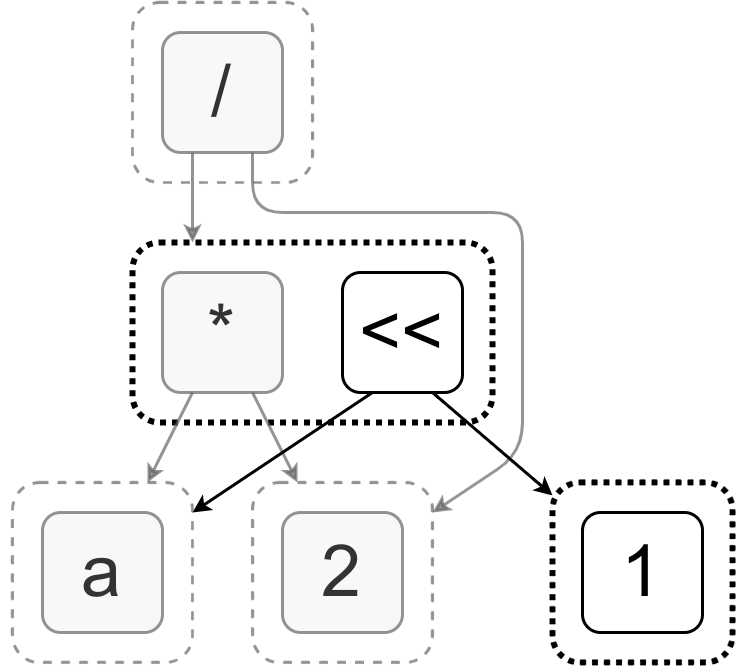
\includegraphics[width=0.44\textwidth]{img/egraph.png}
    \caption{An e-graph with 5 e-classes and 6 e-nodes.}\label{fig:egraph}
\end{wrapfigure}

E-graphs cannot reason on their own: one needs to define the notions of
equality unique to their problem domain. To continue with the example of
computer arithmetic, we could declare properties, like commutativity,
associativity, and distributivity, with \textit{rewrite rules}. For example,
the syntax \texttt{?a + ?b => ?b + ?a} would encode commutativity as a rewrite
rule. The left-hand side denotes a pattern to search for in the e-graph, and
the right side encodes the application of the rule. If the right-hand side of a
rule already exists in the e-graph, its e-class will be merged with the e-class
matched from the left-hand side. Otherwise, the application is inserted as a
new node in the e-class. It is important that rewrite rules are atomic. If a
rule can be broken down into multiple smaller rules, they should. This way you
can better rationalize what types of expression topologies are reachable by
your e-graph.

When using e-graphs to drive a compiler, you place your starting
expression/circuit in an empty e-graph, and each node starts alone in its
e-class. Then, you use the collection of rewrite rules to grow and build the
e-graph with alternative representations. When rewrite rules no longer
introduce new information into the graph, we say we have reach \textit{equality
    saturation}. In many cases, such as Boolean circuits, it is not possible to
fully saturated the e-graph. Instead, a time limit or size limit is reached.
Once the e-graph is built, all that is left is to extract the best rewriting of
the expression. This of course is the NP-hard part. There are several research
projects on e-graph extraction~\cite{smoothe,sparsextract}, but they are beyond
the scope of this course project. However, previous work on FPGA technology
mapping has demonstrated that fast, greedy extraction algorithms can be used
and still find area and circuit depth improvements.

In the end, e-graph driven compilers are less heuristic than conventional
compiler architectures, because they transform terms non-destructively. Typical
optimizing compilers are broken down into a pass pipeline, and the quality of
results is sensitive to the ordering of these optimization passes. Optimizing
compilers built around passes will never be able to generalize to all programs,
but in practice the results are adequate. In the hardware domain, the rules of
economies of scale apply, and the end of transistor scaling makes design
contraints that much tighter. As a solution, e-graphs are a more formal and
more optimal approach to problems in electronic design automation. Previous
work~\cite{esyn} has demonstrated the usefulness of e-graphs for logic
synthesis. Moreover, I hope to submit my own e-graph work to ICCAD which shows
12\% area savings over vendor tools on FPGA applications without increasing
circuit depth.

\section{Experiments}\label{sec:experiments}

Each experiment should describe the motivation, the baseline, the methods, and
evaluation technique. As well as the state of the art.

0. Equivalence Checking and Fuzzing

2. Standard cell development

3. Re-synthesis
- For depth
- For area
- flip flop area

The proposal should be maybe 2-3 pages. It should be a step towards the
introduction for the final project report. So you should include a paragraph or
two about the motivation for the project, a paragraph or two that describes
your plan for the baseline and alternative design, a paragraph or two that
describes how you plan to test and evaluate your design, and a few paragraphs
for the literature review. Your annotated bibliography should go at the end.
Note -- you must annotate at least three scholarly references, but you do not
need to annotate every reference. Feel free to include as many references as
you like. You can find project ideas and more information about the literature
search in the Project Ideas handout on the Canvas handouts page.

\bibliographystyle{plain}
\bibliography{references}

\end{document}